\begin{frame}{FFJORD: Free-Form Continuous Dynamics for Scalable Reversible Generative Models}
    \begin{itemize}
        \item Reversible generative models train using maximum log-likelihood with the change of variable rule.
            \begin{itemize}
                \item Exact PDF
                \item Restrictions on architecture due to determinant calculation.
            \end{itemize}
        \item IDEA: Use Jacobian trace instead
            \begin{itemize}
                \item Transformations specified by Ordinary Differential Equations.
                \item Log-density is now an estimate.
                \item Removes restrictions on architecture, hence "Free-Form".
            \end{itemize}
    \end{itemize}
\end{frame}
\begin{frame}{FFJORD: Continuous Normalizing Flows}
\begin{itemize}
    \item Base distribution $\mathbf{z}_0 \sim p_{z_0}(\mathbf{z}_0)$
    \item ODE defined parametric function $f(\mathbf{z}(t), t; \theta)$
    \item Instantaneous change of variable formula:
    \begin{align*}
        \frac{\partial \text{log} p(\mathbf{z}(t))}{\partial t} = - \text{Tr}(\frac{\partial f}{\partial \mathbf{z}(t)})
    \end{align*}
    \item Change in log-density across time:
    \begin{align*}
        \mathbf{z}(t_0) &= \mathbf{z}_0\\
        \mathbf{z}(t_1) &= f(\mathbf{z}(t_0)) \longrightarrow \text{use with numerical solver}\\
        \text{log} p(\mathbf{z}(t_1)) &= \text{log} p(\mathbf{z}(t_0)) - \int^{t_1}_{t_0}Tr(\frac{\partial f}{\partial \mathbf{z}(t)})
    \end{align*}
\end{itemize}
\end{frame}
\begin{frame}{FFJORD: Scalable density evaluation}
\begin{itemize}
    \item Switching to continuous NF allows for more expressive architectures
    \begin{itemize}
        \item Reduces computational bottleneck from $\mathcal{O}(D^3)$ to $\mathcal{O}(D^2)$
        \item However, introduces numerical ODE solver
    \end{itemize}
    \item Use trace estimate to further reduce the cost:
    \begin{align*}
        Tr(A) = \mathbb{E}_{p(\epsilon)}[\mathbf{\epsilon}^T A \mathbf{\epsilon}] \longrightarrow \text{Hunchinson's trace estimator}
    \end{align*}
    \item $\mathbf{\epsilon}$ is a noise vector such that $\mathbb{E}[\epsilon] = 0$ and $Cov(\epsilon) = 1$
    \begin{align*}
        \text{log} p(\mathbf{z}(t_1)) &= \text{log} p(\mathbf{z}(t_0)) - \mathbb{E}_{p(\epsilon)}[\int^{t_1}_{t_0} \epsilon^T \frac{\partial f}{\partial \mathbf{z}(t)} \epsilon \; dt]
    \end{align*}
\end{itemize}
\end{frame}
\begin{frame}{FFJORD: Complexity}
\begin{itemize}
    \item Cost of evaluating $f$ is $\mathcal{O}(DH)$ where $D$ dimensionality and $H$ size of largest hidden dimension in $f$
    \item DNF - $\mathcal{O}((DH+D^3)L)$ where $L$ \# of layers used
    \item CNF - $\mathcal{O}((DH+D^2)\hat{L})$ where $\hat{L}$ \# evaluations of ODE solver
    \item FFJORD - $\mathcal{O}((DH+D)\hat{L})$
\end{itemize}
\end{frame}
\begin{frame}{FFJORD: Algorithm}
\begin{figure}
    \centering
    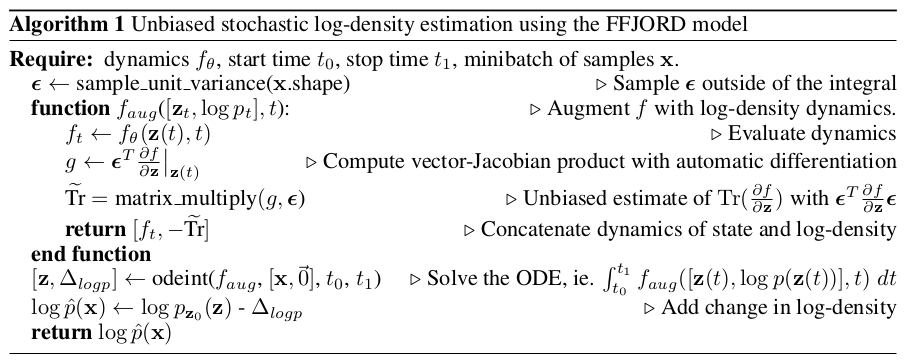
\includegraphics[width=\textwidth, height=8cm,keepaspectratio]{images/ffjord_algorithm.png}
    \label{fig:ffjord_experiments1}
\end{figure}
\end{frame}
\begin{frame}{FFJORD: Experiments}
\begin{figure}
    \centering
    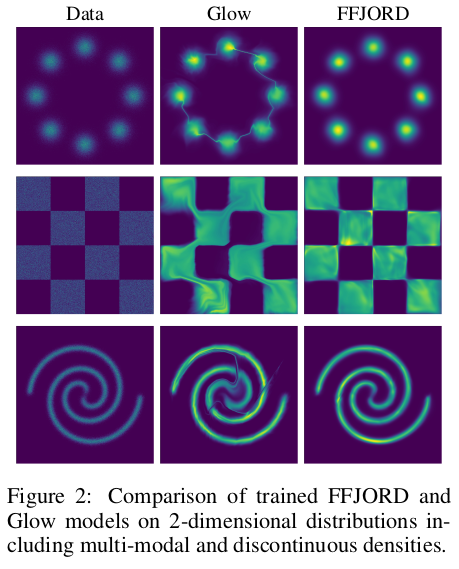
\includegraphics[width=\textwidth,height=8cm, keepaspectratio]{images/ffjord_experiments1.png}
    \label{fig:ffjord_experiments1}
\end{figure}
\end{frame}
\begin{frame}{FFJORD: Experiments}
\begin{figure}
    \centering
    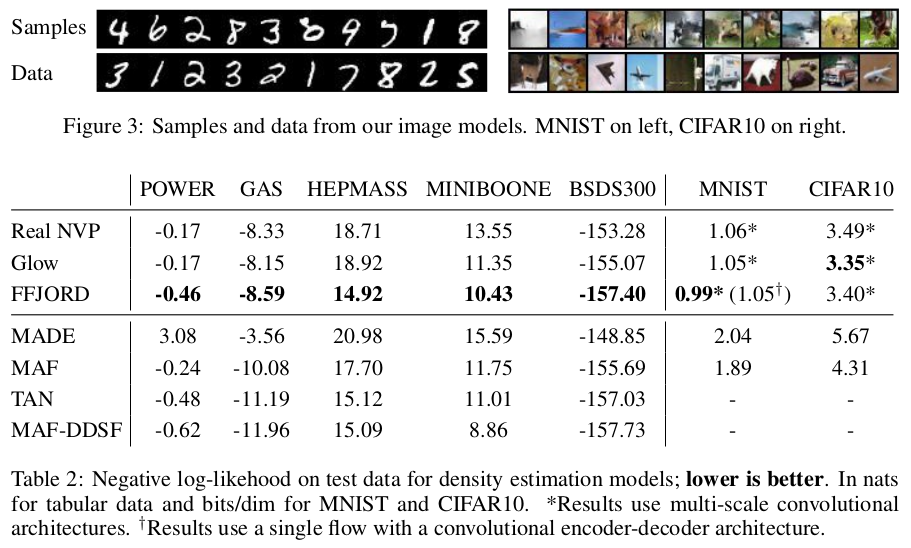
\includegraphics[width=\textwidth,height=8cm, keepaspectratio]{images/ffjord_experiments2.png}
    \label{fig:ffjord_experiments2}
\end{figure}
\end{frame}
\begin{frame}{FFJORD: Comparisons}
    \begin{itemize}
        \item FFJORD outperforms Glow on toy data where it is able to fit multi-modal and discontinuous distributions
            \begin{itemize}
                \item Glow seems to struggle with disconnected regions
            \end{itemize}
        \item On MNIST, FFJORD performs as well as RealNVP and Glow using a single flow and outperforms them using multiscale.
        \item Glow still outperforms FFJORD on CIFAR-10.
            \item However, FFJORD has less parameters and uses a fixed gaussian as prior, instead of a learned distribution.
        \item FFJORD is slower but more memory-efficient.
    \end{itemize}
\end{frame}
\begin{frame}{FFJORD: Limitations}
    \begin{itemize}
        \item Prohibitive number of ODE solver evaluations.
        \begin{itemize}
            \item It's a function of the data, model architecture and parameters.
            \item Increases as the model trains.
        \end{itemize}
        \item General-purpose ODE solvers have restrictions.
    \end{itemize}
\end{frame}
